%BeginMC
\question
Which of the six numbered corresponds to the most recent common ancestor of a mushroom and a sponge?
\begin{multicols}{2}

\begin{choices}
\choice 1. %EndChoice
\choice 2. %EndChoice
\choice 3. %EndChoice
\choice 4. %EndChoice
\correctchoice 5. %EndChoice
\choice 6. %EndChoice
\end{choices}

\columnbreak

	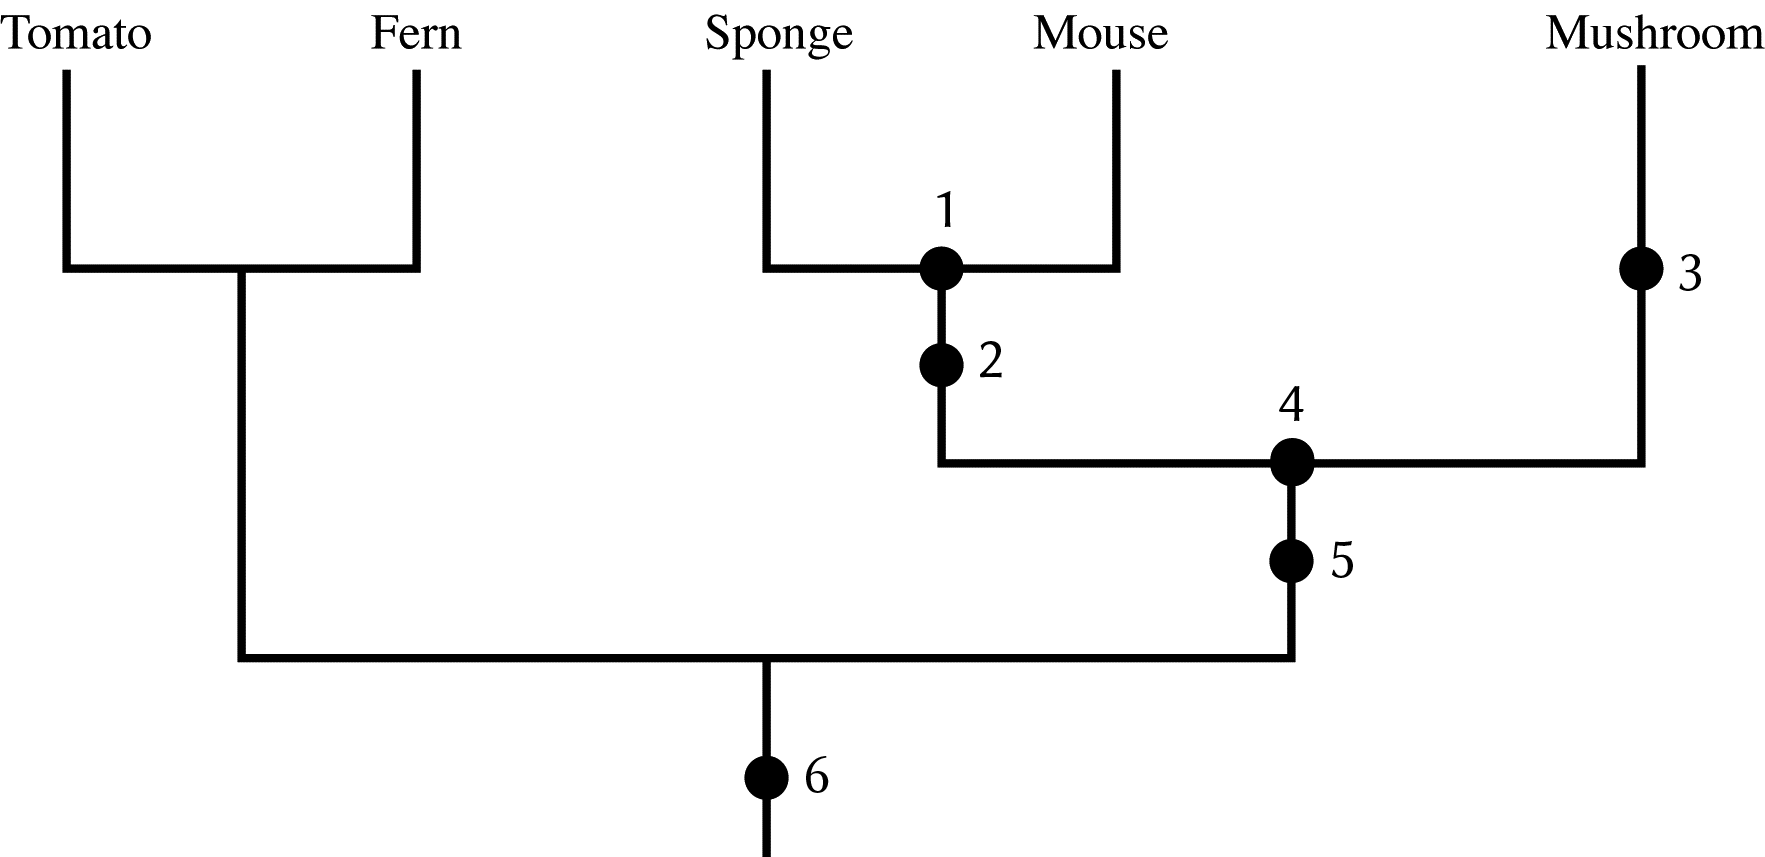
\includegraphics[width=0.45\textwidth]{exam1_tree2}
\end{multicols}
%EndMC

%BeginMC
\question
The oldest fossil remains of \textit{Homo sapiens} found so far date from about  

\begin{choices}
\choice 6 million years ago.   %EndChoice
\choice 1.6 million years ago.   %EndChoice
\correctchoice 200,000 years ago.   %EndChoice
\choice 60,000 years ago.   %EndChoice
\choice 16,000 years ago.  %EndChoice
\end{choices}
%EndMC


%BeginMC
\question
Bird guides once listed the Myrtle Warbler and Audubon's Warbler as distinct species. Recently, these birds have been classified as eastern and western forms of the Yellow-Rumped Warbler. Which one of the following pieces of evidence, if true, would be cause for this reclassification?

\begin{choices}
\correctchoice The two forms interbreed often in nature, and their offspring survive and reproduce well.    %EndChoice
\choice The two forms live in similar habitats and have similar food requirements.   %EndChoice
\choice The two forms have many genes in common.   %EndChoice
\choice The two forms are morphologically similar.   %EndChoice
\choice The two forms overlap for a small part of their their geographic ranges.   %EndChoice
\end{choices}
%EndMC


%BeginMC
\question
Male frogs give calls that attract female frogs to approach and mate. Researchers examined mating calls of closely related tree frogs in South America. If reinforcement is occurring, what would you expect if you compare the calls of the two species in zones of sympatry versus zones of allopatry? 

\begin{choices}
\correctchoice Calls would be more different in areas of sympatry. %EndChoice
\choice Calls would be about the same in both areas. %EndChoice
\choice Calls would be more similar in areas of sympatry. %EndChoice
\choice Calls would become more similar due to fusion. %EndChoice
\choice Calls would show they were cryptic species. %EndChoice
\end{choices}
%EndMC

%BeginMC
\question
A hybrid zone is properly defined as 

\begin{choices}
\correctchoice an area where mating occurs between members of two closely related species, producing at least some viable offspring. %EndChoice
\choice an area where the ranges of two closely related species overlap, but do not interbreed. %EndChoice
\choice a zone where the two closely related species remain distinct through hybrid fusion. %EndChoice
\choice an area where members of two closely related species intermingle, but gene flow is prevented by prezygotic barriers. %EndChoice
\choice an area where members of two closely related species intermingle, but gene flow is prevented by allopatric barriers. %EndChoice
\end{choices}
%EndMC

%BeginMC
\question
What does the biological species concept use as the primary criterion for determining whether two populations are the same species?

\begin{choices}
\correctchoice Gene flow.   %EndChoice
\choice Geographic isolation.   %EndChoice
\choice Ecological differences.   %EndChoice
\choice Morphological similarity.   %EndChoice
\choice Allopatric speciation.   %EndChoice
\end{choices}
%EndMC

%BeginMC
\question
Which of the following factors would \emph{not} contribute to allopatric speciation?

\begin{choices}
\correctchoice Gene flow between the two populations is extensive.   %EndChoice
\choice The separate population is small, and genetic drift occurs.   %EndChoice
\choice One population is exposed to different selection pressures than the other population.   %EndChoice
\choice Different mutations begin to distinguish the gene pools of the separated populations.   %EndChoice
\end{choices}
%EndMC

%BeginMC
\question
Males of different species of fruit fly \textit{Drosophila} that live in the same parts of the Hawaiian Islands have different elaborate courtship rituals. These rituals involve fighting other males and making stylized movements that attract females. What type of reproductive isolation does this represent?

\begin{choices}
\correctchoice Behavioral isolation.   %EndChoice
\choice Gametic isolation.   %EndChoice
\choice Habitat isolation.   %EndChoice
\choice Temporal isolation.   %EndChoice
\choice Mechanical isolation.   %EndChoice
\end{choices}
%EndMC

%BeginMC
\question
Most insects have two pairs of wings. Flies only have one pair of wings. The second pair of wings is reduced to tiny structures called halteres. The mutation(s) that led to the change from wings to halteres could have

\begin{choices}
\correctchoice  altered the expression of a \emph{Hox} gene. %EndChoice
\choice duplicated all of the \emph{Hox} genes in the fly genome. %EndChoice
\choice resulted in paedomorphosis. %EndChoice
\choice caused the loss of \textit{Antp} or . %EndChoice
\choice caused expression of a pseudogene. %EndChoice
\end{choices}
%EndMC

%BeginMC
\question
The most important feature that permits a gene to act as a molecular clock is 

\begin{choices}
\correctchoice a relatively consistent average rate of mutation. %EndChoice
\choice a large number of base pairs. %EndChoice
\choice favored by natural selection. %EndChoice
\choice a recent gene duplication event. %EndChoice
\choice that it is a conserved gene. %EndChoice
\end{choices}
%EndMC


